\documentclass[14pt]{extarticle}

\usepackage{homeworktemplate}
\usepackage[askip=3mm, bskip=3mm]{terminal}
\usepackage[askip=3mm, bskip=3mm]{mylisting}
\usepackage{xurl}
\usepackage{tcolorbox}
\usepackage{xltabular}
\usepackage{array}
\usepackage{pdflscape}
\usepackage{everypage}
\usepackage{csquotes}

\renewcommand{\arraystretch}{1.2}

\newcommand{\Lpagenumber}{\ifdim\textwidth=\linewidth\else\bgroup
  \dimendef\margin=0 %use \margin instead of \dimen0
  \ifodd\value{page}\margin=\oddsidemargin
  \else\margin=\evensidemargin
  \fi
  \raisebox{\dimexpr -\topmargin-\headheight-\headsep-0.5\linewidth}[0pt][0pt]{%
    \rlap{\hspace{\dimexpr \margin+\textheight+\footskip}%
    \llap{\rotatebox{90}{\thepage}}}}%
\egroup\fi}
\AddEverypageHook{\Lpagenumber}%

\title{Домашняя работа 2 \\ Git \& GitHub}

\begin{document}

\maketitle

\tableofcontents

\section{Создание и настройка аккаунта GitHub}

    Для проверки домашних работ необходимо будет создавать
    удаленные Git-репозитории с кодом на платформе
    \href{https://github.com/}{GitHub}.
    Создание репозиториев требует обязательной регистрации.

    \begin{tcolorbox}
        \textbf{Инструкция для создания GitHub аккаунта
        \footnote{Изменить язык инструкции можно в правом верхнем углу веб-интерфейса.}}: \\
        \url{https://docs.github.com/en/get-started/start-your-journey/creating-an-account-on-github}.
    \end{tcolorbox}

    Имя и почта пользователя, указанные при создании аккаунта, потребуются далее.

    Обратите внимание, что создать GitHub аккаунт нельзя с почтой из домена
    \verb|ru| (т.е., \verb|@mail.ru|, \verb|@yandex.ru| и др.).
    Для регистрации необходимо использовать или имеющийся почтовый ящик из другого
    домена, или создать его.
    Хорошими вариантами будут почтовые ящики \verb|@gmail.com| или \verb|@outlook.com|.

    \subsection{Добавление SSH-ключа}

        Команды клиента Git, работающие с удаленным репозиторием (например,
        \verb|git push| или \verb|git pull|), должны аутентифицировать пользователя
        для проверки, может ли он выполнять операции чтения или записи содержимого
        репозитория.
        Аутентифицироваться можно двумя способами: по логину и паролю и с использованием
        пары SSH-ключей.

        Аутентификация с логином и паролем требует их ввод после \textit{каждой}
        команды, работающей с удаленным репозиторием.
        Это не очень удобно.

        Аутентификация при помощи пары SSH-ключей требует однократного добавления
        приватного SSH-ключа в GitHub аккаунт.

        \begin{tcolorbox}
            \textbf{Инструкции для создания и добавления SSH-ключа}: \\
            \begin{enumerate}
                \item \url{https://docs.github.com/en/authentication/connecting-to-github-with-ssh/generating-a-new-ssh-key-and-adding-it-to-the-ssh-agent?platform=linux}
                \item \url{https://docs.github.com/en/authentication/connecting-to-github-with-ssh/adding-a-new-ssh-key-to-your-github-account}
            \end{enumerate}
        \end{tcolorbox}

\section{Установка и настройка клиента Git}

    \subsection{Установка}

        Клиент Git может быть уже установлен в систему.
        В командной строке введите:

        \begin{terminalwindow}
!\shellcommand{git --version}!
        \end{terminalwindow}

        Если в выводе команды есть версия клиента Git, то установка не требуется.
        В ином случае следуйте шагам по установке:

        \begin{enumerate}

            \item Если текущий пользователь --- не суперпользователь (root),
                выполните команду смены пользователя (потребуется пароль
                суперпользователя).

                \begin{terminalwindow}
!\shellcommand{su -}!
                \end{terminalwindow}

            \item Выполните команду установки клиента Git.

                \begin{terminalwindow}
!\shellcommand{apt-get install -y git}!
                \end{terminalwindow}

            \item Выполните команду завершения сессии суперпользователя.

                \begin{terminalwindow}
!\shellcommand{exit}!
                \end{terminalwindow}

        \end{enumerate}

    \subsection{Настройка}

        При создании коммитов клиенту Git необходимо имя пользователя и его почтовый
        ящик.
        Пусть \verb|<USERNAME>| и \verb|<EMAIL>| --- имя и почта пользователя,
        указанные при создании аккаунта GitHub.
        Выполните команды:

        \begin{terminalwindow}
!\shellcommand{git config --global user.name <USERNAME>}!
!\shellcommand{git config --global user.email <EMAIL>}!
        \end{terminalwindow}

\section{Форк репозитория}

    В домашнем задании вам необходимо написать код в собственной копии
    репозитория \url{https://github.com/czertyaka/CppDevCourse-hw2}.
    Такая копия в большинстве сервисов хостинга Git-репозиториев
    (таких как GitHub, BitBucket и др.) называется \textbf{форком}
    \footnote{\url{https://docs.github.com/en/pull-requests/collaborating-with-pull-requests/working-with-forks/fork-a-repo\#about-forks}}
    (fork).

    В этом разделе вы выполните следующие шаги:

    \begin{enumerate}
        \item cоздадите форк репозитория \texttt{CppDevCourse-hw2};
        \item склонируете собственный форк;
        \item добавите файл \textit{main.cpp};
        \item протестируете корректность добавленного кода;
        \item отправите свои изменения в удаленный Git-репозиторий.
    \end{enumerate}

    \subsection{Создание форка репозитория}

    Создайте форк репозитория \url{https://github.com/czertyaka/CppDevCourse-hw2}
    согласно инструкции по ссылке ниже.

    \begin{tcolorbox}
        \textbf{Инструкция для создания форка репозитория}: \\
        \url{https://docs.github.com/en/pull-requests/collaborating-with-pull-requests/working-with-forks/fork-a-repo}.
    \end{tcolorbox}

    \subsection{Клонирование форка репозитория}

    В веб-интерфейсе GitHub получите адрес для клонирования вашего форка.
    Обратите внимание, что нужно выбрать адрес для клонирования с использолванием
    ключей SSH.

    \begin{tcolorbox}
        \textbf{Инструкция для клонирования репозитория}: \\
        \url{https://docs.github.com/en/repositories/creating-and-managing-repositories/cloning-a-repository}.
    \end{tcolorbox}

    Получив адрес \verb|<ADDRESS>|, выполните команды:

    \begin{terminalwindow}
!\shellcommand{git clone <ADDRESS>}!
!\shellcommand{cd CppDevCourse-hw2/}!
    \end{terminalwindow}

    Убедитесь в корректности проделанных действий, выполнив команду \verb|ls -a1|
    для вывода содержимого директории CppDevCourse-hw2.
    Вывод команды должен совпадать с выводом ниже:

    \begin{terminalwindow}
!\shellcommand{ls -a1}!
./
../
CMakeLists.txt
.git/
.github/
README.md
test.py
    \end{terminalwindow}

    \subsection{Добавление и тестирование кода}

    В директории проекта создайте файл \textit{main.cpp} с простейшей программой,
    выводящей в консоль строку \verb|"Hello, World!"| с символом новой строки в конце.

    Убедитесь, что проект корректно собирается:

    \begin{terminalwindow}
!\shellcommand{cmake -B build}!
!\shellcommand{cmake --build build}!
    \end{terminalwindow}

    Протестируйте собранное приложение:

    \begin{terminalwindow}[||]
|\shellcommand{./build/main}|
Hello, World!
|\shellcommand{ctest --test-dir build}|
    Start 1: main
1/1 Test #1: main .....................   Passed    0.04 sec

100% tests passed, 0 tests failed out of 1

Total Test time (real) =   0.04 sec
    \end{terminalwindow}

    \subsection{Отправка изменений}

    Добавьте созданный файл \textit{main.cpp} в индекс Git, создайте коммит
    с сообщением \enquote{added main.cpp} и отправьте изменения в форк:

    \begin{terminalwindow}
!\shellcommand{git add main.cpp}!
!\shellcommand{git commit -m "added main.cpp"}!
!\shellcommand{git push}!
    \end{terminalwindow}

    Вывод команды \verb|git status| должен быть похож на:

    \begin{terminalwindow}
!\shellcommand{git status}!
On branch master
Your branch is up to date with 'origin/master'.

Untracked files:
  (use "git add <file>..." to include in what will be committed)
        build/

nothing added to commit but untracked files present (use "git add" to track)
    \end{terminalwindow}

\section{Пулл-реквест}

    Из форка\footnotemark{} в оригинальный репозиторий можно создать \textbf{запрос на слияние}
    (в англоязычных источниках pull-request или merge-request).
    Пулл-реквест позволяет разработчику исходного репозитория обозревать изменения,
    сделанные в форке, комментировать их, и, в конечном счете, либо соглашаться с ними,
    добавляя эти изменения в исходный репозиторий, либо отказываться от них.

    \footnotetext{Пулл-реквесты можно создать и внутри одного проекта из одной
    \href{https://git-scm.com/book/en/v2/Git-Branching-Branches-in-a-Nutshell}{ветки}
    в другую.}

    Создайте пулл-реквест из вашего форка в репозиторий
    \url{https://github.com/czertyaka/CppDevCourse-hw2}.
    Названием пулл-реквеста должны быть ФИО студента.

    \begin{tcolorbox}
        \textbf{Инструкция по созданию пулл-реквеста в GitHub}: \\
        \url{https://docs.github.com/en/pull-requests/collaborating-with-pull-requests/proposing-changes-to-your-work-with-pull-requests/creating-a-pull-request-from-a-fork}.
    \end{tcolorbox}

    В веб-интерфейсе на странице пулл-реквеста доступны несколько вкладок:

    \begin{itemize}

        \item \textit{Conversation}. На этой вкладке видна история работы в пулл-реквесте:
            добавление новых коммитов после открытия репозитория, комментарии
            преподавателя и студента, результаты автоматических проверок и статус
            пулл-реквеста.

        \item \textit{Commits}. В этой вкладке можно найти список коммитов, которые
            были созданы после создания форка.

        \item \textit{Checks}. В этой вкладке находятся подробности выполнения
            последней автоматизированной проверки.

        \item \textit{Files changed}. В этой вкладке можно посмотреть все изменения
            в пулл-реквесте.
            Убедитесь, что в вашем пулл-реквесте нет других изменений, кроме
            добавленного файла \textit{main.cpp}.

    \end{itemize}

    Домашнее задание считается выполненным, если:

    \begin{enumerate}

        \item пулл-реквест успешно создан;

        \item в названии пулл-реквеста есть ФИО студента;

        \item нет других изменений в пулл-реквесте, кроме добавленного файла
            \textit{main.cpp};

        \item пулл-реквест прошел автоматизированную проверку (во вкладке
            \textit{Conversation} есть статус \enquote{All checks have passed}).

    \end{enumerate}

    На рис.~\ref{fig:pr} скриншот правильно выполненного и оформленного пулл-реквеста.

    \begin{figure}[ht]
        \centering
        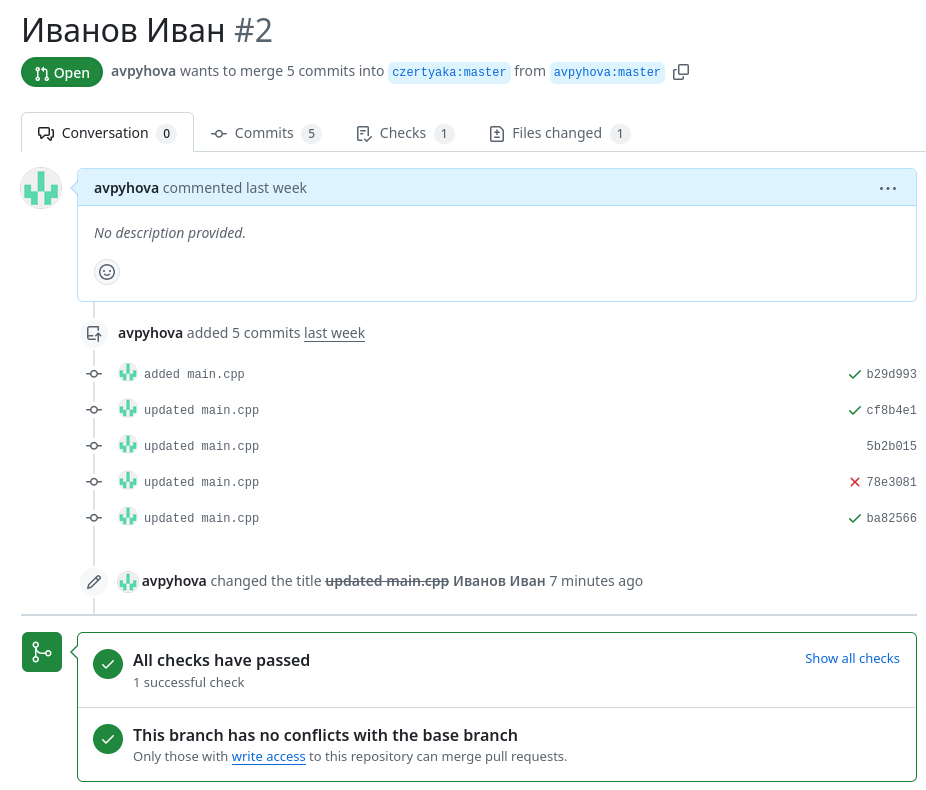
\includegraphics[width=\textwidth]{Homeworks/02-Git/pull-request.png}
        \caption{Пример успешно выполненного домашнего задания.}
        \label{fig:pr}
    \end{figure}

\clearpage

\begin{landscape}

\pagestyle{empty}

\appendix

\section{Cheat sheet команд Git}

    \begin{xltabular}{\linewidth}{|X|X|}

        \hline
        \textbf{Команда} & \textbf{Описание} \\
        \hline
        \hline
        \endfirsthead

        \hline
        \textbf{Команда} & \textbf{Описание} \\
        \hline
        \hline
        \endhead

        \hline
        \endfoot

        \hline
        \endlastfoot

        \verb|git status| &
        Посмотреть текущее состояние рабочей директории и индекса. \\
        \hline
        \verb|git add [FILE ...]| &
        Добавить файл(ы) в индекс Git, например, \verb|git add main.cpp foo.cpp|. \\
        \hline
        \verb|git commit [-m "<MESSAGE>"]| &
        Создать коммит. При использовании флага \verb|-m| возможно установить
        сообщение в коммите, например: \hfill \break
        \verb|git commit -m "added main.cpp"|. \\
        \hline
        \verb|git push| &
        Отправить изменения из ветку локального репозитория в ветку
        удаленного репозитория. \\
        \hline
        \verb|git fetch| &
        Скачать информацию о ветках в удаленном репозитории. \\
        \hline
        \verb|git pull| &
        Влить ветку из удаленного репозитория в ветку
        локального репозитория. \\
        \hline
        \verb|git show [<COMMIT>]| &
        Показать информацию о коммите.
        Если не указывать хэш коммита \verb|COMMIT|, то будет показана
        информация о текущем коммите. \\
        \hline
        \verb|git log [--oneline --graph --decorate]| &
        Показать историю коммитов текущей ветки.
        Флаги \verb|--oneline --graph --decorate| сделают историю короче
        и читаемее. \\
        \hline
        \verb|git restore [--staged] <FILE> ...| &
        Обратить изменения в рабочей директории (без флага \verb|--staged|)
        или в индексе (с флагом \verb|--staged|).
        Примеры: \hfill \break
        \verb|git restore main.cpp foo.cpp| \hfill \break
        \verb|git restore --staged foo.h|. \\
        \hline
        \verb|git checkout [-b] <BRANCH>| &
        Переключиться на ветку \verb|BRANCH|.
        Если используется флаг \verb|b| и ветки \verb|BRANCH| не существует,
        то она будет создана.
        Примеры: \hfill \break
        \verb|git checkout master| \hfill \break
        \verb|git checkout -b feature|. \\

    \end{xltabular}

    Материалы для самостоятельного изучения:

    \begin{itemize}

        \item Git Pro Book:
            \url{https://git-scm.com/book/ru/v2}.

        \item Онлайн-тренажер LearnGitBranching:
            \url{https://learngitbranching.js.org/?locale=ru\_RU}.
    \end{itemize}

\end{landscape}

\end{document}
